% Interpretabilidad SHAP
\section{Interpretabilidad}

\begin{frame}
\frametitle{¿Por qué SHAP?}
\textbf{Problema}: el GBM es una caja gris. Sin interpretabilidad, no es útil para política pública.

\vspace{0.3cm}
\textbf{SHAP (Lundberg \& Lee, 2017)}: descompone cada predicción como suma de contribuciones por variable.

\vspace{0.2cm}
\textit{Propiedad clave}: aditividad
\[
f(x_i) = \phi_0 + \sum_j \phi_{ij}
\]

\vspace{0.2cm}
La importancia global es $\text{Imp}_j = \mathbb{E}[\,|\phi_j|\,]$.
\end{frame}

\begin{frame}
\frametitle{Importancia SHAP — global (modelo ampliado)}
\centering
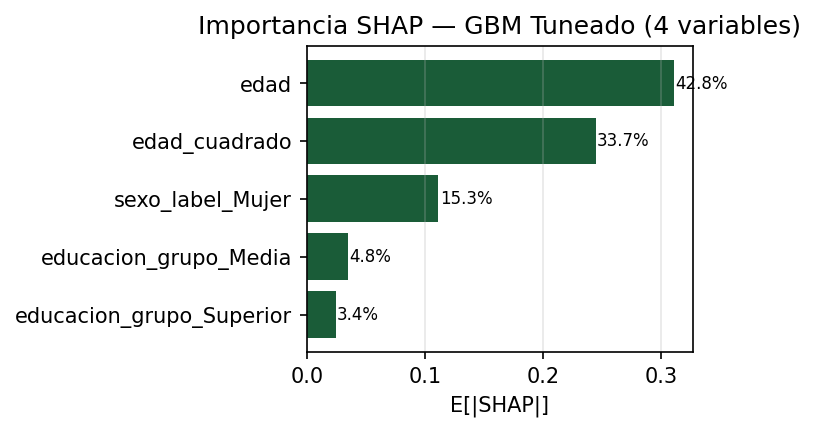
\includegraphics[width=0.78\textwidth]{../figures/shap_bar.png}
\\
\vspace{0.2cm}
\small Con 4 features: edad + edad² ${\sim}77\%$, sexo 15\%, educación 8\% — modelo demográfico puro.\\
Con 16 features: se espera que \texttt{amigos\_consumen}, \texttt{probaria\_sustancias} y \texttt{riesgo\_marihuana\_ocasional} ganen peso. Ver notebook 06 para el análisis actualizado.
\end{frame}

\begin{frame}
\frametitle{SHAP summary — distribución individual}
\centering
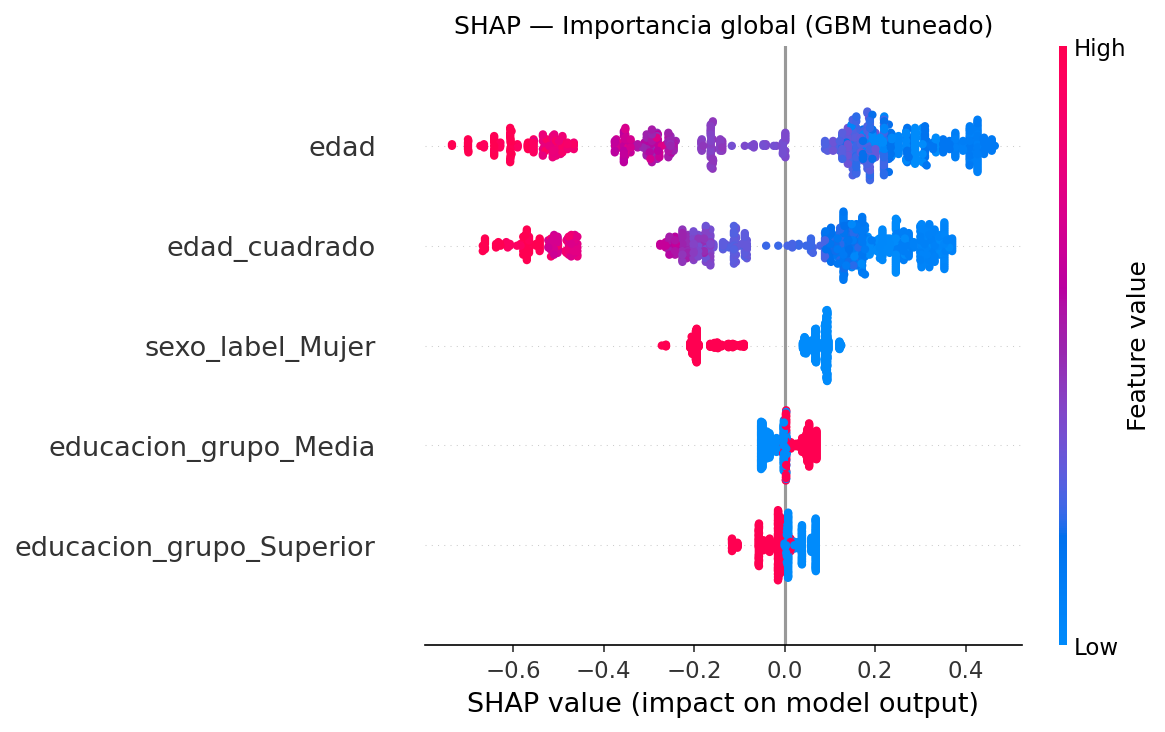
\includegraphics[height=0.78\textheight,keepaspectratio]{../figures/shap_summary.png}
\end{frame}

\begin{frame}
\frametitle{Dependencia parcial — edad}
\centering
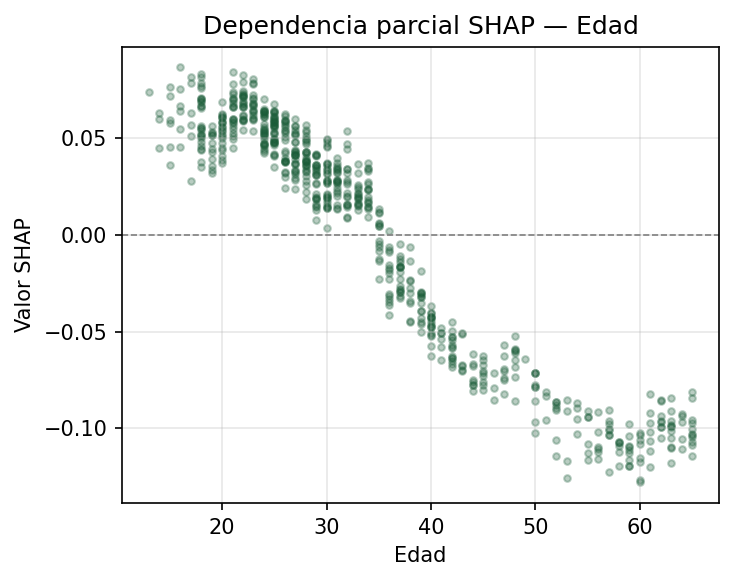
\includegraphics[height=0.66\textheight,keepaspectratio]{../figures/shap_dependence_edad.png}
\\
\vspace{0.05cm}
\scriptsize Relación no monótona: positiva en jóvenes, decae con la edad. Por qué gana el GBM: captura mejor esta forma funcional que el lineal.
\end{frame}

\begin{frame}
\frametitle{Robustez — Y alternativa estricta}
\small
\textbf{Motivación}: la auditoría detectó que \texttt{consumo\_12m} difiere de \texttt{K\_03} en 898 casos.

\vspace{0.2cm}
\textbf{Test}: reentrenar el GBM tuneado con $Y_{\text{alt}}=\mathbb{1}\{K\_03=1\}$.

\vspace{0.2cm}
\centering
\footnotesize
\begin{tabular}{lrrr}
\toprule
Métrica & Y original & Y estricta & $\Delta$ \\
\midrule
AUC-ROC (test)        & 0.7182 & 0.6870 & $-0.031$ \\
CV AUC-10fold (mean)  & 0.6685 & 0.6951 & $+0.027$ \\
\bottomrule
\end{tabular}
\vspace{0.25cm}
\\
\flushleft
\scriptsize\textbf{Conclusión}: las relaciones estructurales se mantienen; la discrepancia no domina el resultado.
\end{frame}
